%************************************************
\chapter{Comportamento termico}\label{chp:ComportamentoTermico}
%************************************************
Per andare ad analizzare il comportamento termico di un materiale polimerico consideriamo uno completamente amorfo, per il momento. 
Alla figura \ref{fig:Tg}, viene rappresentato il suo comportamento termico.
\graffito{All'aumentare della temperatura, dopo la transizione vetrosa, il materiale abbasserà ulteriormente il suo modulo elastico fino ad arrivare alla condizione di fluido ad alta viscosità}
Dal grafico si rilevano due zone separate dalla temperatura di transizione vetrosa $T_g$.
La prima zona si chiama di \textbf{vetro} ed è la zona in cui il materiale polimerico amorfo presenta il suo massimo modulo elastico.
Nella seconda zona invece si definisce a comportamento \textbf{gomma} in cui il materiale perde la sua caratteristica di modulo elastico, fino ad arrivare alla condizione di fluido ad alta viscosità.

\begin{figure}
\centering
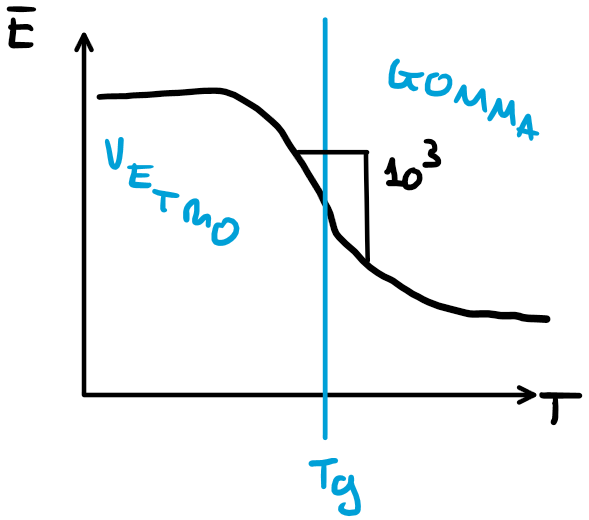
\includegraphics[width = \textwidth]{gfx/Tg}
\caption{Comportamento termico di un materiale amorfo}
\label{fig:Tg}
\end{figure}


Nella realtà, la transizione vetrosa avviene all'interno di un determinato range di temperature. Per convenzione viene fissato la temperatura intermedia a tale range.
A livello microstrutturale non c'è un vero e proprio cambio di struttura nel materiale perché il materiale amorfo era e amorfo rimane.

\begin{figure}
\centering
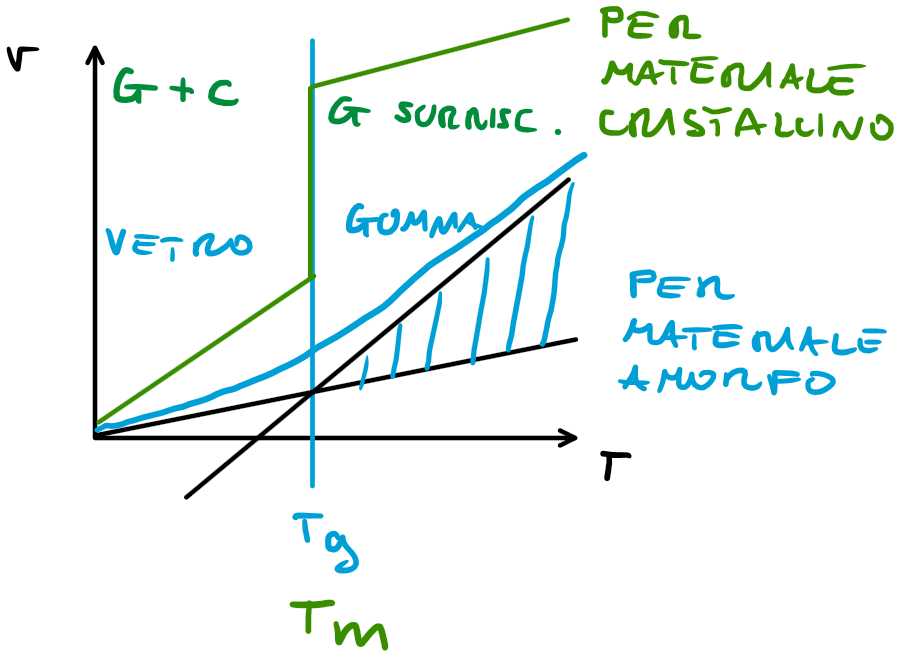
\includegraphics[width = \textwidth]{gfx/VolSpec}
\caption{In termini di volume specifico si vedono in comportamenti per un materiale amorfo e uno semicristallino}
\label{fig:VolSpec}
\end{figure}

Il grafico mostrato in figura \ref{fig:VolSpec}, presenta la variazione del volume specifico in funzione della temperatura sia per un materiale amorfo che per un materiale semi cristallino.
Ciò che accade è che al passaggio attraverso la temperatura di transizione vetrosa $T_g$ aumenta lo spazio libero tra una molecola e l'altra. Determinando, così, una maggiore capacità delle molecole di vibrare attorno ad un punto di equilibrio. Ciò determina anche la repentina diminuzione del modulo elastico. 
Modificando la pressione esterna il comportamento viene traslato verso temperature maggiori, questo perché la pressione limita la vibrazione delle molecole quindi serve più energia per poter ottenere lo stesso comportamento. 

\begin{quote}
\emph{Per un materiale semicristallino?}
\end{quote}


\begin{figure}
\centering
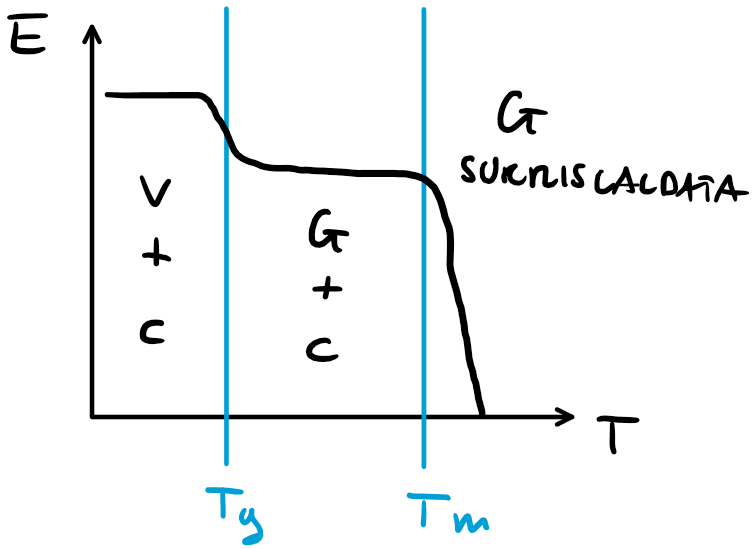
\includegraphics[width = \textwidth]{gfx/TgTm}
\caption{Comportamento termico di un materiale semicristallino}
\label{fig:TgTm}
\end{figure}
Nei materiali semicristallini si ha una vera e propria trasformazione di fase in questo caso si ha una temperatura specifica di trasformazione.

La temperatura di fusione $T_m$ è un unico valore per cui il materiale può essere tranquillamente lavorabile. 
A differenza dei materiali amorfi, la transizione tra materiale cristallino e fluido non risente della pressione in quanto i cristalli sono già compatti.
Dunque, non presentano gli stessi fenomeni evidenziati precedentemente.
 
Per gli amorfi si preferisce oltrepassare il plateau di stato di gomma e avere un materiale molto fluido.
I materiali amorfi vengono utilizzati sempre allo stato vetroso mai gommoso. Sono, tendenzialmente, rigidi e abbastanza resistenti ma fragili. La gomma invece è tendenzialmente duttile e lavorabile.
I materiali cristallini, invece, se utilizzati sotto la temperatura di transizione vetrosa $T_g$ sarebbero materiali eccessivamente fragili. Risulta più conveniente usare all'interno della temperatura di transazione vetrosa e quella di fusione $T_g < T < T_m$. Si ha una gomma rinforzata da cristalli la parte amorfa conferisce tenacità, mentre i cristalli le proprietà meccaniche. 

In generale le plastiche trasparenti sono sempre allo stato vetroso, infatti sono amorfe e di conseguenza fragili. Fa eccezione il \ac{PC} che è a morfo ma non è fragile.
Gli elastomeri sono delle gomme reticolate, per cui conservano le loro proprietà per un buon tratto oltre la temperatura di fusione per via della reticolazione quindi non fondono.

\section{Fattori che influenzano la transizione}
La transizione vetrosa è influenzata da:
\begin{itemize}
\item Mobilità della catena principale,
\item Sostituenti laterali: ingombro e mobilità propria,
\item Legami intermolecolare,
\item Peso molecolare.
\end{itemize}

\paragraph{Mobilità della catena principale}
La transizione vetrosa dipende dalla vibrazione delle molecole attorno alla loro posizione di equilibrio: dunque per catene molto mobili si ha una temperatura di transizione vetrosa più bassa.
Per esempio il \ac{PE} ha una transizione vetrosa a $-100\unit{\celsius}$, decisamente bassa.   
Incrementando la rigidezza della catena polimerica la temperatura di transizione vetrosa aumenta.
Altri materiali:
\begin{itemize}
\item il \ac{PET} ha $T_g = 60\unit{\celsius}$,
\item il \ac{PC} ha $T_g = 120\unit{\celsius}$.
\end{itemize}

\begin{quote}
\emph{Come mai il \ac{PET} lo usiamo a temperatura ambiente anche se risulterebbe vetroso?}
\end{quote}
In questo caso è molto importante il fattore acqua contenuta nell'umidità ambientale.
Tale comportamento, figura \ref{fig:Umidita}, è dovuto ai legami intermolecolari deboli tra le varie catene in cui l'acqua si va ad inserire in mezzo ai legami intermolecolari realizzando una specie di "lubrificazione" tra le molecole. Viene detto \textbf{effetto plastificante}. L'acqua plastifica il polimero, di fatto spezza i legami intermolecolari.
Diminuendo il numero di legami intermolecolari ancora in atto si va a diminuire la temperatura di transizione vetrosa permettendo alle molecole di essere libere a minore energia. 

\begin{figure}
\centering
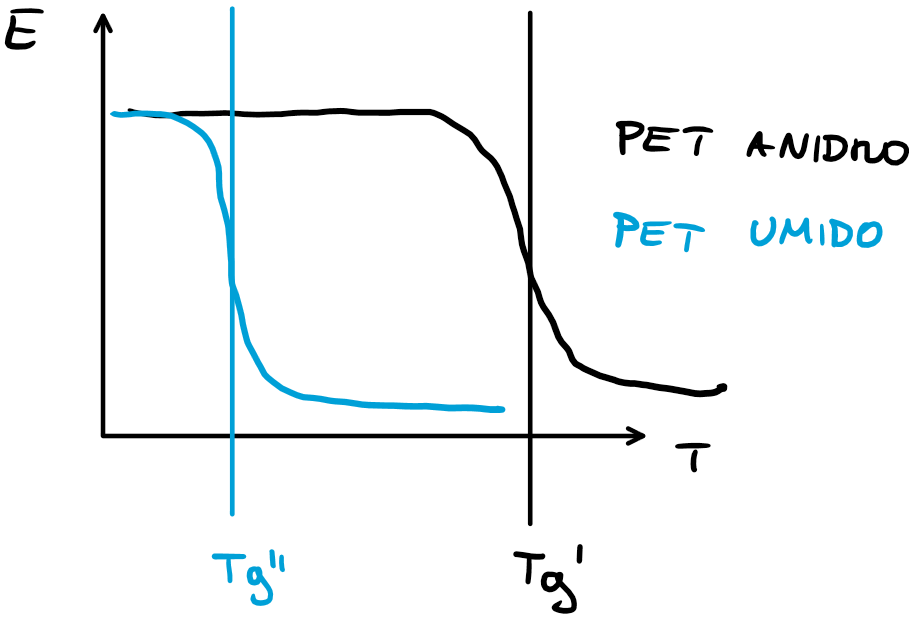
\includegraphics[width = \textwidth]{gfx/Umidita}
\caption{Effetto di abbassamento della transizione per via dell'umidità}
\label{fig:Umidita}
\end{figure}

\paragraph{Sostituenti laterali}
Un sostituente particolarmente ingombrante porta un incremento notevole della $T_g$. Se, per esempio, consideriamo un anello benzenico la temperatura viene aumentata da $-100\unit{\celsius}$ del \ac{PP} a $100\unit{\celsius}$ del \ac{PS}. Mostrati in figura \ref{fig:ConfPPPS}.

\begin{figure}
\centering
\subfloat[][\emph{}\label{fig:PP}]
{%
\begin{minipage}[b]{0.4\textwidth}
\setchemfig{atom sep = 2em}
\schemestart
\chemname{\chemfig{\vphantom{C}-[@{op,.5}]C(-[2]CH_3)(-[6]H)-C(-[2]H)(-[6]H)-[@{cl,.5}]}}{Polipropilene}
\polymerdelim[delimiters ={[]}, indice = n]{op}{cl}
\schemestop
\end{minipage}%
}\quad
\subfloat[][\emph{}\label{fig:PS}]
{%
\begin{minipage}[b]{0.4\textwidth}
\setchemfig{atom sep = 2em}
\schemestart
\chemname{\chemfig{\vphantom{C}-[@{op,.5}]C(-[2]**6(------))(-[6]H)-C(-[2]H)(-[6]H)-[@{cl,.5}]}}{Polistirene}
\polymerdelim[delimiters ={[]}, indice = n]{op}{cl}
\schemestop
\end{minipage}%
}
\caption{Confronto tra i monomeri di polipropilene e polistirene}
\label{fig:ConfPPPS}
\end{figure}

Si può osservare che pur aumentando l'ingombro, se la catena sostituente è molto mobile allora gli effetti si sovrappongono. Il punto è che la mobilità crea molto più volume libero. Dunque l'effetto diventa contrario rispetto a mettere un semplice sostituente. Questo perché bisogna considerare sia il fattore di ingombro che il fattore di mobilità del sostituente in cui la mobilità del sostituente gioca un ruolo più importante.

\paragraph{Legami intermolecolari}
I legami intermolecolari più aumentano in termini di forza e frequenza più la temperatura di transizione vetrosa $T_g$ aumenterà.
Ad esempio il \ac{PVC}, questo genera dei legami intermolecolari più forti. Infatti ha una transizione vetrosa più alta rispetto al polipropilene nonostante siano entrambi materiali vinilici. 

\paragraph{Peso molecolare}
Come era stato anticipato precedentemente, il peso molecolare influisce molto sulla temperatura di transizione vetrosa. Infatti molecole ad alto grado di polimerizzazione avranno sicuramente un peso molecolare più alto ma necessitano di maggiore energia cinetica per potersi muovere.
Siccome necessitano di maggiore energia vuol dire che la temperatura di transizione vetrosa verrà spostata verso valori più alti rispetto a molecole che avendo un grado di polimerizzazione più basso necessiteranno di minore energia per agitarsi.
Risulta essere tutta una questione cinetica.

%************************************************
\chapter{Viscoelasticità}\label{ch:viscoelasticità}
%************************************************
Si tratta della caratterizzazione del comportamento meccanico delle plastiche allo stato solido.

Ipotizzando un materiale solido di cui non si conoscono le caratteristiche meccaniche, la prima prova che si fa è la prova di trazione: si tira e si vede cosa succede.

\begin{quote}
\emph{Si, ma\dots \dots non funziona come per i metalli}
\end{quote}
Infatti si presenta uno sforzo dipendente, si dal carico, anche dalla velocità di deformazione.
In generale, i materiali plastici hanno una forte \textbf{sensibilità alla velocità di deformazione}.
Non è l'unica deviazione dal comportamento dai solidi metallici.

Se un materiale è elastico, allora determinato il modulo elastico, o modulo di Young, si conosce il materiale.
Per le plastiche vale diversamente: se il materiale è completamente amorfo, allora effettivamente l'analisi del modulo elastico è molto significativa per il materiale. Questo però è un caso limite, da non prendere come regola generale.
Dunque, questo tipo di prova non è significativa per i materiali polimerici.

Si preferisce caratterizzarli in altro modo:
\begin{equation}
\sigma = \sigma(\epsilon,\dot{\epsilon})
\end{equation}
ovvero lo sforzo non è determinato solo dalla deformazione ma anche dalla \textbf{velocità di deformazione}.

Allora per caratterizzare il materiale è opportuno misurare proprio le deviazione dal comportamento elastico:
\begin{itemize}
\item Scorrimento viscoso \textbf{Creep},
\item Rilassamento degli sforzi.
\end{itemize}

\paragraph{Rilassamento degli sforzi}
Viene imposta una deformazione costante nel tempo.
Va ricordato che:
\begin{equation}
\epsilon = \frac{L - L_0}{L_0} \quad	\sigma = e(\dot{\epsilon},t)
\end{equation}
Allora il comportamento che si osserva per tale prova è quello delle figure \ref{fig:RilassamentoE} e \ref{fig:RilassamentoS}.

\begin{figure}
\centering
\subfloat[][\emph{Imposizione della deformazione costante}\label{fig:RilassamentoE}]
{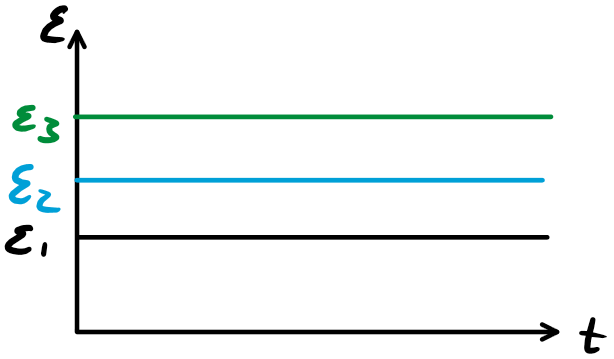
\includegraphics[width = 0.4\textwidth]{gfx/RilassamentoE}}\quad
\subfloat[][\emph{Fenomeno del rilassamento degli sforzi}\label{fig:RilassamentoS}]
{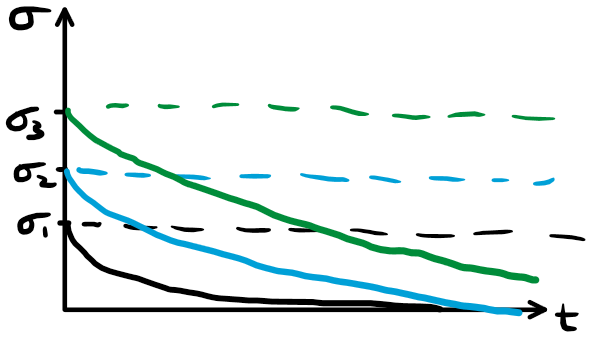
\includegraphics[width = 0.4\textwidth]{gfx/RilassamentoS}}\\
\subfloat[][\emph{Imposizione dello sforzo costante}\label{fig:CreepS}]
{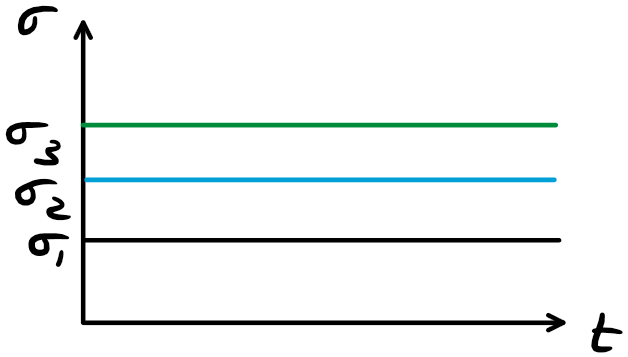
\includegraphics[width = 0.4\textwidth]{gfx/CreepS}}\quad
\subfloat[][\emph{Effetto di \eng{Creep}}\label{fig:CreepE}]
{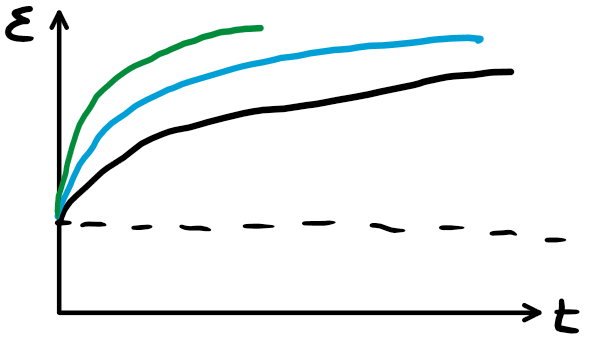
\includegraphics[width = 0.4\textwidth]{gfx/CreepE}}
\end{figure}

\paragraph{Scorrimento viscoso (\eng{Creep})}
Imponendo uno sforzo costante, si osserva l'andamento della deformazione del materiale.

Se la risposta del materiale è lineare, in una delle due variabili, allora la caratterizzazione del materiale può essere più semplice. Sopratutto de il primo degli argomenti di $\bar{\epsilon}$ o $\bar{\sigma}$.

Affinché una funzione sia lineare deve soddisfare entrambe le seguenti:
\begin{align}
f(k*x) &= kf(x) :=\textup{Condizione di funzione omogenea}\\
f(x_1 + x_2) &= f(x_1) + f(x_2) :=\textup{Principio di sovrapposizone degli effetti}
\end{align}

\section{Viscoelasticità lineare}
Ricordando che:
\begin{equation}
\begin{split}
\sigma &= e(\bar{\epsilon}, t) &=\textup{Rilassamento}\label{eqn:Rilassamento}%
\\
\epsilon &= d(\bar{\sigma}, t) &=\textup{\eng{Creep}}
\end{split}
\end{equation}
Ipotizzando che $e$ sia lineare in $\bar{\epsilon}$:
\begin{equation}
e(\bar{\epsilon},t) \rightarrow \bar{\epsilon} * E(t)
\label{eqn:ModuloRilassamento}
\end{equation}
Dove si può definire $E(t)$ come \textbf{Modulo di rilassamento}.
Lo si può ottenere sostituendo nella \eqref{eqn:Rilassamento} la definizione appena trovata \eqref{eqn:ModuloRilassamento}, ottenendo:
\begin{equation}
E(t) = \frac{\sigma(t)}{\bar{\epsilon}}
\end{equation}
Ciò vale solamente in cui il materiale sia linearmente dipendente dalla deformazione.
D'altra parte si può definire un comportamento analogo nel caso:
\begin{equation}
\epsilon(t) = d(\bar{\sigma},t) = \bar{\sigma} * D(t)
\end{equation}
Allora si può definire $D(t)$ come \textbf{Cedevolezza di creep}.
Definito, in maniera analoga al modulo di rilassamento:
\begin{equation}
D(t) = \frac{\epsilon(t)}{\bar{\sigma}}
\end{equation}
Sempre a patto che il materiale presenti una dipendenza lineare allo sforzo applicato.

Valgono anche le seguenti:
\begin{enumerate}
\item Se il materiale è lineare in rilassamento, allora lo è anche in \eng{creep}. Se il materiale è lineare in \eng{creep} allora lo è anche in rilassamento.
\item $E(t)$ e $D(t)$ non sono indipendenti tra loro: misurandone una si ottiene di conseguenza l'altra. Il problema sta nella complessità della relazione tra le due.
\item Misurando tutte e due, si può ottenere il comportamento del materiale anche quando una delle due "costanti" è funzione del tempo. Dunque considerando una storia sforzo/carico arbitraria.
\end{enumerate}
Quindi: il materiale o è lineare o non lo è e non c'è modo di linearizzarlo.

Con le ipotesi di linearità con risposta viscoelastica del materiale,
le equazioni che abbiamo trovato sono:
\begin{align}
\sigma(t) &= E(t)\epsilon_0 + \int_0^t{E(t-s)\dot{\epsilon}(s)\,ds} \label{eqn:RilassamentoComp}\\
\epsilon(t) &= D(t)\sigma_0 + \int_0^t{D(t-s)\dot{\sigma}(s)\,ds}\label{eqn:CreepCompleto}
\end{align}

\subsection{Test per la valutazione se il materiale è lineare}
Le equazioni viste precedentemente evidenziano come il materiale si deformi in maniera lineare, ma il contributo totale è rappresentato da un primo contributo iniziale e poi la storia di deformazione del materiale.

Per valutare la linearità della risposta viscoelastica si va a valutare solamente l'omogeneità della funzione.

Per ipotesi immaginiamo un test di \eng{creep}. Allora per verificare la linearità si fruttano le curve \textbf{isocrone}. 
Si considera un determinato tempo $\bar{t}$ al quale corrisponderà sia un certo carico (costante), sia una certa deformazione che si ottiene tramite le curve di deformazione al \eng{creep}. Si prendono quei valori e li si graficano in una coppia d'assi $\epsilon-\sigma$ come in figura \ref{fig:Isocrone}.

\begin{figure}
\centering
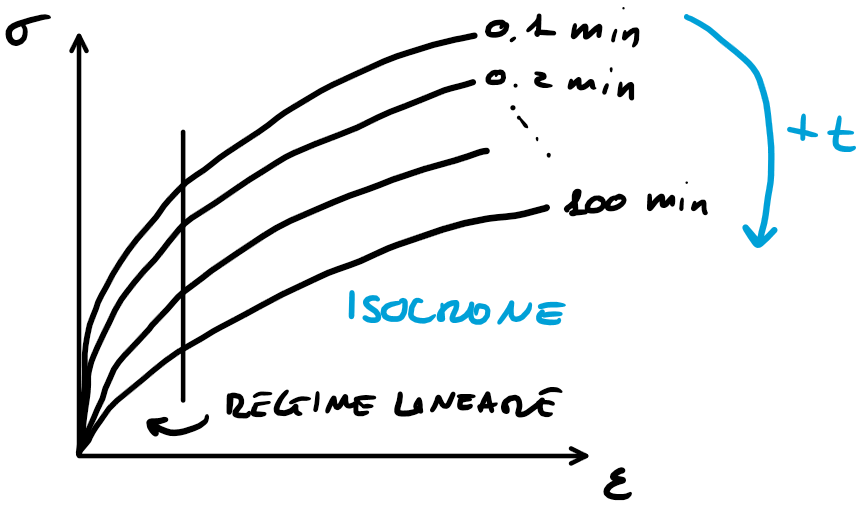
\includegraphics[width = \textwidth]{gfx/Isocrone}
\caption{Schematizzazione delle curve isocrone prese a partire da una prova di \eng{creep}}
\label{fig:Isocrone}
\end{figure}

\paragraph{Osservazioni}
\begin{itemize}
\item Si sarebbe tentati di considerarle delle prove di trazione: ovviamente non lo sono, la modalità di realizzazione è completamente diversa da una mera prova di trazione.
\item Siccome vale:
\begin{equation}
\epsilon(t) = \sigma_iD(t) \rightarrow \epsilon(\bar{t}) = \sigma_iD(t)
\end{equation}
In più \begin{equation}
\frac{\sigma_i}{\epsilon(\bar{t})} = \frac{1}{D(\bar{t})}
\end{equation}
evidenziando come la funzione di effettivamente lineare. Dunque, rappresentabile tramite semirette.
\item Inoltre, come approssimazione ingegneristica, le isocrone ottenute tramite \eng{creep} o come rilassamento siano le stesse. In realtà non è propriamente vero.
\end{itemize}

Come si vede dal grafico \ref{fig:Isocrone}, effettivamente le isocrone non sono propriamente lineari: per deformazioni/sforzi molto alti ci si rende conto del comportamento meno che lineare.
Allora, di solito, si considera che ad una deformazione del $1\% \div 1.5\%$ se le isocrone sono approssimativamente rettilinee, allora il materiale ha comportamento viscoelastico lineare.

Nel caso si vogliano le isocrone a partire da una prova di rilassamento:
\begin{equation}
\begin{split}
\sigma(t) &= \epsilon_iE(t) \rightarrow \sigma(\bar{t}) = \epsilon_iE(\bar{t})\\
\frac{\sigma(\bar{t})}{\epsilon_i} &= E(\bar{t}) = cost.
\end{split}
\end{equation}

\section{Prova di trazione per materiali viscoelastici lineari}
Si impone una deformazione a velocità costante, si misura lo sforzo: $\epsilon(t) = \alpha t$.
In cui $\alpha$ è la \textbf{velocità di deformazione} imposta.
ricordando che:
\begin{equation}
\begin{split}
\sigma(t) &= E(t)\epsilon_0 + \int_0^t{E(t-s)*\dot{\epsilon}(s)\,ds}\\
&=E(t)\epsilon_0 + \int_0^t{E(t-s)*\alpha\,ds} =E(t)\epsilon_0 + \alpha \int_0^t{E(t-s)\,ds}\\
&\Rightarrow \underbrace{\left[t-s = \tau\right]}_{\textup{Cambio variabile}} \Rightarrow\\
&=E(t)\epsilon_0 + \alpha \int_t^0{E(\tau)\,(-d\tau)} = E(t)\epsilon_0 + \alpha \int_0^t{E(\tau)\,d\tau}\\
&= E(t)\epsilon_0 + \alpha \int_0^t{E(s)\,ds}\\
\sigma &= \sigma(t) \rightarrow \sigma = \sigma(\epsilon)
\end{split}
\end{equation}
Dunque, per ottenere lo sforzo in funzione della deformazione:
\begin{equation}
\begin{split}
\epsilon &= \alpha * t \rightarrow t = \epsilon/\alpha\\
\sigma &= \sigma\left(\frac{\epsilon}{\alpha}\right)\\
\sigma &= \alpha \int_0^t{E(s)\,ds}
\end{split}
\end{equation}
Per sapere, indicativamente l'andamento dello sforzo:
\begin{equation}
\begin{split}
\frac{d\sigma}{d\epsilon} = \alpha\frac{d\int}{dE} = \alpha \frac{d\int}{d\frac{\epsilon}{\alpha}}*\frac{d\frac{\epsilon}{\alpha}}{dE}
\end{split}
\end{equation}
Per un materiale viscoelastico lineare presenta un grafico sforzo-deformazione crescente lineare non rettilineo, molto simile alle isocrone senza che lo sia.
la curva di può parametrizzare si $\alpha$ che, in un certo senso, rappresenta il tempo nel caso delle isocrone. In realtà, aumentando la velocità di deformazione il materiale presenta un comportamento più rigido.
\begin{equation}
E_y = \frac{d\sigma}{d\epsilon}\Big|_{\epsilon = 0} = E(0)
\end{equation}
Ci dice che la rigidezza rimane sempre la stessa al variare della velocità do deformazione.
\begin{equation}
\begin{split}
E_y &= \frac{\bar{\sigma}}{\bar{\epsilon}} = \frac{1}{\bar{\epsilon}}\int_0^{\bar{\epsilon}/\alpha}{E(s)\,ds}\\
&= \int_0^{\bar{\epsilon}/\alpha}{E(s)\,ds} - E(\bar{\epsilon}/\alpha) * \bar{\epsilon}/\alpha
\end{split}
\end{equation}

Materiali che sono viscoelastici hanno un comportamento intermedio tra quello di un fluido e quello di un solido. Il comportamento è tipico delle plastiche allo stato solido.

\section{Fluidi e solidi viscoelastici}
Un fluido viscoelastico ha un modulo di rilassamento pari a 0. Per cui dato uno sforzo, il fluido andrà a deformazione permanente.
Un solido viscoelastico, al contrario, ha modulo di rilassamento finale strettamente positivo.

$D_0$ è legato all'elasticità istantanea che si verifica per tempi relativamente brevi. Se il materiale è un solido viscoelastico, la risposta sarà vincolata ad un asintoto orizzontale.
Se invece è un fluido visco elastico, la sua risposta non è limitata, per cui la cedevolezza di \eng{creep} non è limitata superiormente.

%************************************************
\chapter{Legame tra modulo di rilassamento e cedevolezza di \eng{creep}}%
\label{chp:LegameCedevolezzaCreep}
%************************************************
\section{Prova di \eng{creep}}
Da un punto di vista dimensionale sono l'uno il reciproco dell'altro.
\begin{equation}
\sigma(t) = E(t)\epsilon_0 + \int_0^t{E(t-s)*\dot{\epsilon}(s)\,ds}
\end{equation}
Questa vale anche nel caso della prova di \eng{creep}: lo sforzo sarà costante:
\begin{equation}
\sigma(t) = \bar{\sigma} \qquad \epsilon(t) = \bar{\sigma} D(t)
\end{equation}
Dunque:
\begin{equation}
\begin{split}
\bar{\sigma} &= E(t) * \bar{\sigma} * D(0) + \int_0^t{E(t-s)\bar{\sigma}\dot{D}(s)\,ds}\\
1 &= E(t) * D(0) + \int_0^t{E(t-s)\dot{s}\,ds}
\end{split}
\end{equation}
Eventuali approssimazioni:
\begin{equation}
t \rightarrow 0
\end{equation}
Allora:
\begin{equation}
1 = E(0) * D(0) \rightarrow E(0) = \frac{1}{D(0)}
\end{equation}
Il comportamento di questo materiale è elastico: prevale la componente conservativa che non quella dissipativa. per tempi molto piccoli.
Ipotizzando un tempo generico, allora: $E(t-s) > E(t)$ perché la funzione modulo di rilassamento è una funzione decrescente.
\begin{equation}
\begin{split}
1 &= E(t)D(0) + \int_0^t{E(t-s)\dot{D}(s)\,ds}\\
1 &> E(t)D(0) + \int_0^t{E(t)\dot{D}(s)\,ds}\\
&= E(t)D(0) + E(t)[D(t)-D(0)] = E(t) * D(t) \rightarrow D(t) \leq \frac{1}{E(t)}
\end{split}
\end{equation}
Tale conferma anche la condizione precedente, infatti per tempi prossimi a 0 si ha una maggior componente elastica che no dissipativa.

Ora ipotizzando che: $\epsilon(t) = \alpha t$ allora:
\begin{equation}
\begin{split}
\alpha t &= D(t) * 0 + \int_0^t{D(t-s)*\alpha*E(s)\,ds}\\
t &= \int_0^t{D(t-s)E(s)\,ds}
\end{split}
\end{equation}
Siccome $D(t-s) \leq D(t)$ perché è una funzione crescente come si vede in figura \ref{fig:Creep}
\begin{figure}
\centering
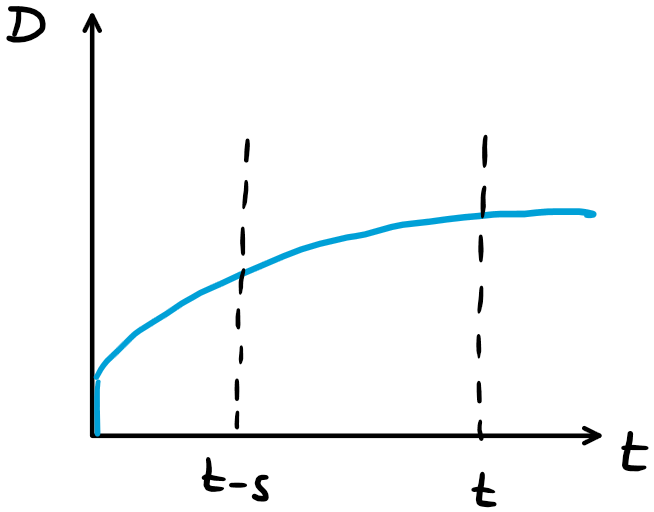
\includegraphics[width = 0.5\textwidth]{gfx/Creep}
\caption{Approssimazione dell'andamento del \eng{creep} per un materiale viscoelastico}
\label{fig:Creep}
\end{figure}
Allora resta valido:
\begin{equation}
t = \int_0^t{D(t-s)E(s)\,ds} \leq \int_0^t{D(t)E(s)\,ds} = D(t)\int_0^t{E(s)\,ds}
\end{equation}
Da cui
\begin{equation}
D(t) \geq \frac{t}{\int_0^t{E(s)\,ds}}
\end{equation}
Lo si può anche scrivere come:
\begin{equation}
D(t) \geq \frac{1}{\underbrace{\frac{1}{t}\int_0^t{E(s)\,ds}}_{\textup{è un valore medio}}}
\end{equation}
Dunque:
\begin{equation}
\begin{split}
\frac{1}{\frac{1}{t}\int_0^t{E(s)\,ds}} \leq D(t) \leq \frac{1}{E(t)}\\
\frac{1}{\bar{E}} \leq D(t) \leq \frac{1}{E(t)}
\end{split}
\end{equation}
Per cui possiamo dire che 
\begin{equation}
D(t) \approx \frac{1}{E(t)}
\end{equation}

Considerando ora $t \rightarrow \infty$: se il materiale è un solido viscoelastico, allora il materiale presenta un asintoto diverso da zero:
\begin{equation}
\exists D_{\infty} < \infty \quad \exists E_{\infty} \neq 0
\end{equation}
Ricordando:
\begin{equation}
\frac{1}{\frac{1}{t}\int_0^t{E(s)\,ds}} \leq D(t) \leq \frac{1}{E(t)}
\end{equation}
Portandolo verso tempi molto lunghi possiamo scrivere che:
\begin{equation}
\frac{\int_0^t{E(s)\,ds}}{t} \, \overrightarrow{t \rightarrow \infty} \, \frac{E(t)}{1}\rightarrow E_{\infty}
\end{equation}
Allora:
\begin{equation}
1 \leq D_{\infty} \leq \frac{1}{E_{\infty}}
\end{equation}

\paragraph{Riassumendo}
Per tempi piccoli il materiale si comporta come se fosse completamente elastico, in quanto cedevolezza e modulo di rilassamento sono l'uno il reciproco dell'altro.
Per tempi intermedi di sforzo ha comportamento viscoelastico.
Per tempi molto più lunghi il materiale si comporterà nuovamente a carattere elastico
\begin{description}
\item[Tempi brevi] \textbf{Comportamento elastico}
\item[Tempi intermedi] \textbf{Comportamento viscoelastico} ovvero ha componente sia elastica che dissipativa.
\item[Tempi lunghi] \textbf{Comportamento elastico}
\end{description}

\section{Prova di rilassamento}
Idealmente saremmo in grado di deformare istantaneamente il materiale, evidentemente ciò non è possibile perché il materiale tende a comportarsi in maniera diversa.
Dunque bisogna utilizzare una rampa di deformazione, da cui si stima il modulo di rilassamento, capendo quanto si sta sbagliando e come.
Allora:
\begin{equation}
\epsilon(t)=%
\begin{cases}
\frac{\bar{\epsilon}}{t}t &0<t<\bar{t}\\
\bar{\epsilon} &t>\bar{t}
\end{cases}
\label{eqn:ProvaRilassamento}
\end{equation}

\begin{figure}
\centering
\subfloat[][\emph{Profilo della deformazione}\label{fig:ProfiloDeformazione}]%
{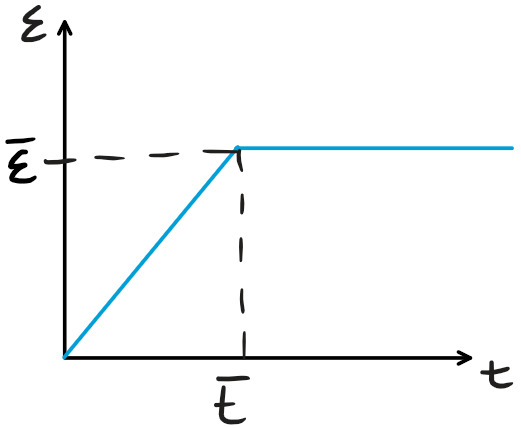
\includegraphics[width = 0.4\textwidth]{gfx/ProfiloDeformazione}}\quad
\subfloat[][\emph{Profilo dello sforzo conseguente}\label{fig:ProfiloSforzo}]%
{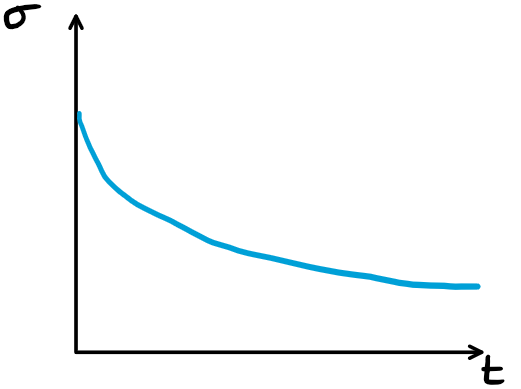
\includegraphics[width = 0.4\textwidth]{gfx/ProfiloSforzo}}	
\caption{Prova di rilassamento}
\label{fig:ProvaRilassamento}
\end{figure}
Conviene separare i due momenti come evidenziato dall'equazione \eqref{eqn:ProvaRilassamento}.

\begin{description}
\item[$0<t<\bar{t}$]
\begin{equation}
\begin{split}
\epsilon(t)&=\frac{\bar{\epsilon}}{\bar{t}}t \quad \dot{\epsilon}=\frac{\bar{\epsilon}}{\bar{t}}\\
\sigma(t)&=\frac{\bar{\epsilon}}{\bar{t}}\int_0^t{E(s)\,ds}\\
\bar{\sigma}(t)&=\sigma(\bar{t})=\frac{\bar{\epsilon}}{\bar{t}}\int_0^{\bar{t}}{E(s)\,ds}
\end{split}
\end{equation}
Il risultato di questo integrale è quello della figura \ref{fig:tMinBar}
\item[$t>\bar{t}$]
\begin{equation}
\begin{split}
\epsilon(t)&=\bar{\epsilon} \quad \dot{\epsilon}(t)=0\\
\sigma(t)&=E(t)\epsilon_0 + \int_0^t{E(t-s)\dot{\epsilon}(s)\,ds}\\
&=\int_0^{\bar{t}}{E(t-s)\dot{\epsilon}(s)\,ds} + \int_{\bar{t}}^t{E(t-s)\dot{\epsilon}(s)\,ds}\\
\sigma(t)&=\int_0^{\bar{t}}{E(t-s)\,ds} \quad\overrightarrow{\tau = t-s}\quad \frac{\bar{\epsilon}}{\bar{t}}\int_t^{t-\bar{t}}{E(\tau)\,(-d\tau)}\\
&= \frac{\bar{\epsilon}}{\bar{t}}\int_{t-\bar{t}}^t{E(s)\,ds}
\end{split}
\end{equation}
Il risultato di questo risultato è \ref{fig:tMagBar}.
\item[$t=\bar{t}$]
\begin{equation}
\begin{split}
\sigma^+(t) &= \frac{\bar{\epsilon}}{\bar{t}}\int_0^{\bar{t}}{E(s)\,ds}\\
\frac{d\sigma}{dt}&=\frac{\bar{\epsilon}}{\bar{t}}(E(t)-E(t-\bar{t}))<0\\
\frac{d^2\sigma}{dt^2}&=\frac{\bar{\epsilon}}{\bar{t}}(\dot{E}(t)-\dot{E}(t-\bar{t})\geq 0\\
\bar{E}(t)&= \frac{\sigma(t)}{\bar{\epsilon}} \quad \leftrightarrow \quad E(t)\\
\bar{E}&=\frac{\sigma(t)}{\bar{\epsilon}} = \frac{1}{\bar{\epsilon}}\frac{\bar{\epsilon}}{\bar{t}}\int_{t-\bar{t}}^t{E(s)\,ds}\\
&=\frac{1}{\bar{t}}\int_{t-\bar{t}}^t{E(s)\,ds}\lesseqgtr E(t)\bar{t}\\
F(t)&\rightarrow \bar{E}(t)-E(t) = \frac{1}{\bar{t}}\int_{t-\bar{t}}^t{E(s)\,ds} - E(t)\\
\frac{dF}{dt} &= \frac{1}{\bar{t}}\left(E(t)-E(t-\bar{t})\right)-\dot{E}(t)<0
\end{split}
\end{equation}
In questo p[unto si vuole dimostrare la continuità della funzione sforzo e si valuta il successivo andamento della continuità come nella figura \ref{fig:tMagBar}.
Inoltre, viene dimostrata dalla figura \ref{fig:ValutazioneEccesso} che l'approssimazione che stiamo seguendo è per eccesso.
In più si osserva che l'errore si assottiglia man mano che si va avanti col tempo, come si vede in figura \ref{fig:ValutazioneErrore}.
Mentre, la figura. \ref{fig:DimostrazioneIntegrali} si fa notare dal punto di vista geometrico il significato dell'ultima riga.
\end{description}

\begin{figure}
\centering
\subfloat[][\emph{Andamento dello sforzo per $0<t<\bar{t}$}\label{fig:tMinBar}]%
{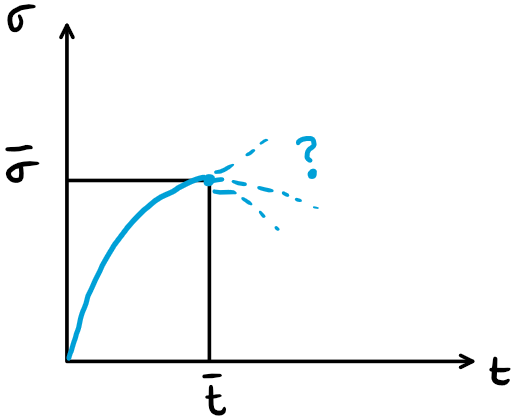
\includegraphics[width = 0.4\textwidth]{gfx/tMinBar}}\quad
\subfloat[][\emph{Andamento dello sforzo per $t>\bar{t}$}\label{fig:tMagBar}]%
{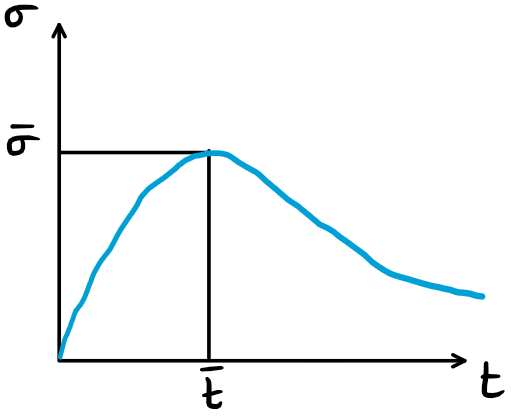
\includegraphics[width = 0.4\textwidth]{gfx/tMagBar}}\\
\subfloat[][\emph{Valutazione dell'errore commesso per via della natura della prova}\label{fig:ValutazioneErrore}]%
{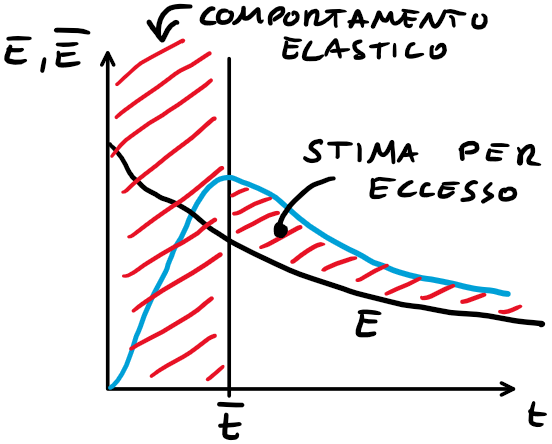
\includegraphics[width = 0.4\textwidth]{gfx/ValutazioneErrore}}\quad
\subfloat[][\emph{Dimostrazione dell'errore per eccesso}\label{fig:ValutazioneEccesso}]%
{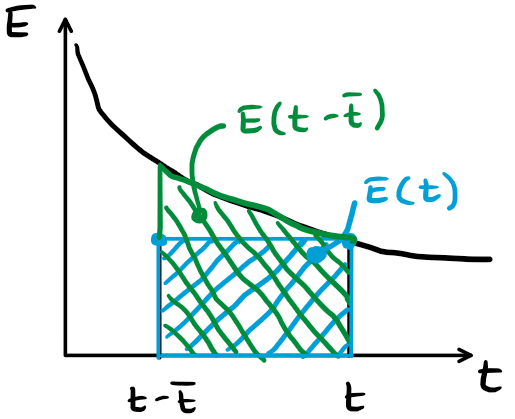
\includegraphics[width = 0.4\textwidth]{gfx/ValutazioneEccesso}}\\
\subfloat[][\emph{Dimostrazione geometrica degli integrali}\label{fig:DimostrazioneIntegrali}]%
{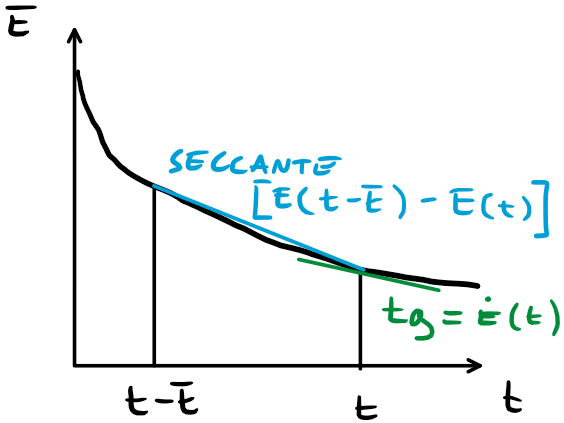
\includegraphics[width = 0.4\textwidth]{gfx/DimostrazioneIntegrale}}	
\caption{Prova di rilassamento reale}
\label{fig:ProvaRilassamento}		
\end{figure}

La prova di rilassamento con rampa, commette un errore per eccesso per via della natura della prova. Per tempi sufficientemente lunghi si abbassa l'effetto dell'errore.
Quando si considerano tempi ben più grandi di quello della rampa (di solito dura qualche secondo) la differenza tra \textbf{stima del modulo di rilassamento} e \textbf{modulo di rilassamento} non è così evidente.
Per avere dei dati per una durata maggiore, si usa alzare la temperatura del materiale. In questo modo si simula il comportamento di ore per una prova di qualche minuto.
Nel caso si vogliano informazioni su anni di esercizio, questi vengono interpolati dalle varie prove.

%************************************************
\chapter{Modelli dei fluidi viscoelastici}\label{chp:ModelliFluidi}
%************************************************
I modelli descritti in letteratura sono una combinazione di elementi \textbf{elastici} e \textbf{dissipativi}.
La viscoelasticità è un comportamento misto, parzialmente elastico e parzialmente dissipativo.
Dunque:
\begin{quote}
\emph{Quando vale il modulo di rilassamento $E(t)$ e il modulo di cedevolezza al \eng{creep} $D(t)$?}
\end{quote}

Allora conviene considerare i due elementi fondamentali:

\begin{figure}
\centering
\subfloat[][\emph{Parametrizzazione come molla per effetti elastici}\label{fig:Molla}]%
{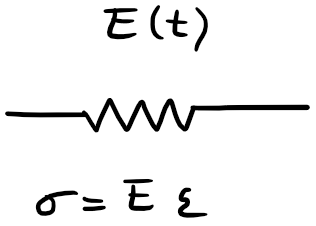
\includegraphics[width = 0.4\textwidth]{gfx/Molla}}\quad
\subfloat[][\emph{Parametrizzazione come smorzatore per gli effetti dissipativi}\label{fig:Dissipatore}]%
{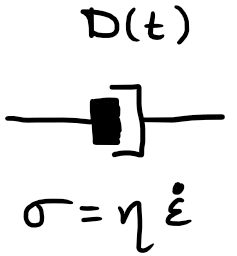
\includegraphics[width = 0.4\textwidth]{gfx/Dissipatore}}	
\caption{Elementi di modellazione dei fluidi viscoelastici}
\label{fig:FluidiViscoelastici}	
\end{figure}

Tra l'altro si vuole ricordare che:
\begin{equation}
\begin{split}
\sigma = \eta \dot{\epsilon} &\textup{Sforzo normale}\\
\tau = \eta \dot{\gamma} &\textup{Sforzo di taglio}
\end{split}
\end{equation}

\section{Fluido di Maxwell}
Rappresentato in figura \ref{fig:FluidoMaxwell}.
\begin{figure}
\centering
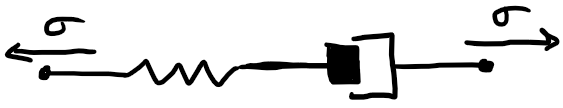
\includegraphics[width = \textwidth]{gfx/FluidoMaxwell}
\caption{Schematizzazione del fluido di Maxwell}
\label{fig:FluidoMaxwell}
\end{figure}

\begin{equation}
\sigma = \sigma_1 = \sigma_2
\end{equation}
Lo sforzo su, rispettivamente, molla e smorzatore.
Mentre la deformazione è:
\begin{equation}
\epsilon = \epsilon_1 + \epsilon_2
\end{equation}
Siccome:
\begin{equation}
\sigma_1 = E*\epsilon_1 \qquad \sigma_2=\eta \dot{\epsilon}_2
\end{equation}
Da cui:
\begin{equation}
\dot{\epsilon} = \dot{\epsilon}_1 + \dot{\epsilon}_2 = \frac{\dot{\sigma}_1}{E} + \frac{\sigma_2}{\eta} = \frac{\dot{\sigma}}{E} + \frac{\sigma}{\eta}
\end{equation}

Dunque:
\begin{equation}
\epsilon = \bar{\epsilon} \rightarrow%
\begin{cases}
\frac{\dot{\sigma}}{E}+\frac{\sigma}{\eta} = 0\\
\sigma_0 = E \cdot \bar{\epsilon}
\end{cases}
\end{equation}
con le seguenti condizioni iniziali:
\begin{equation}
\begin{split}
t&=0\\
\sigma &= E \cdot \bar{\epsilon}
\end{split}
\end{equation}
Risolvendo il sistema di equazioni differenziali:
\begin{equation}
\begin{split}
\frac{d\sigma}{dt} &+ \frac{E}{\eta} \sigma = 0\\
\frac{d\sigma}{dt} &= -\frac{E}{\eta} \sigma \Rightarrow \int{\frac{d\sigma}{\sigma}} = \int{-\frac{E}{t}t}\\
\ln(\sigma)&= -\frac{E}{\eta}t + K \Rightarrow \sigma = e^{-\frac{E}{\eta}t+K}\\
\sigma &= C e^{-\frac{E}{\eta}t}\\
\sigma(0) &= C = E\bar{\epsilon}\\
\sigma(t) &= E\bar{\epsilon}e^{-\frac{E}{\eta}t}\\
E&= \frac{\sigma(t)}{\bar{\epsilon}}=Ee^{-\frac{E}{\eta}t}
\end{split}
\end{equation}
Dove:
\begin{equation}
\tau_r = \frac{\eta}{E} := \textup{ Tempo di rilassamento}
\end{equation}
Da cui infine:
\begin{equation}
E=E_0 e^{-\frac{t}{\tau_r}}
\end{equation}
Il quale comportamento è rappresentato dalla figura \ref{fig:RilassamentoMaxwell}
\begin{figure}
\centering
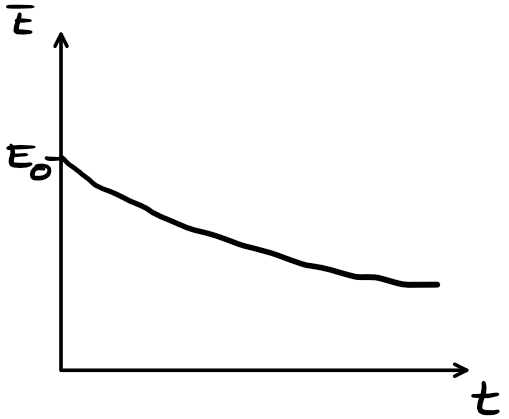
\includegraphics[width = 0.5\textwidth]{gfx/RilassamentoMaxwell}
\caption{Andamento del fluido di Maxwell in termini di rilassamento}
\label{fig:RilassamentoMaxwell}
\end{figure}

Grazie a questi modelli si riesce a capire come funziona anche senza fare calcoli.
Se si tira la molla in serie con un dissipatore, si allunga la molla, ma mano a mano che passa il tempo, tutto il carico preso dalla molla verrà rilassato dal dissipatore viscoso che inizierà a muoversi finché la tensione rimanente verrà rilassata completamente.
La storia di carico è moto prevedibile per via della semplicità del materiale.
\begin{equation}
E(t) = E_0 e^{-\frac{t}{\tau_r}}
\end{equation}
Valutiamo il comportamento al \eng{creep}.
\subsection{Prova di \eng{creep}}
Ricordiamo:
\begin{equation}
\dot{\epsilon} = \frac{\dot{\sigma}}{E} + \frac{\sigma}{\eta}, \quad \sigma = \bar{\sigma} \quad \forall t > 0
\end{equation}
La condizione iniziale:
\begin{equation}
\dot{\epsilon} = \frac{0}{E} + \frac{\bar{\sigma}}{\eta} = \frac{\bar{\sigma}}{\eta} \Rightarrow \epsilon(0)=\frac{\bar{\epsilon}}{E}
\end{equation}
Risolvendo l'equazione differenziale:
\begin{equation}
\epsilon(t) = \frac{\bar{\sigma}}{\eta}t + C \rightarrow \epsilon(0) = \frac{\bar{\sigma}}{E} = C \rightarrow \epsilon(t) = \frac{\bar{\sigma}}{\eta}t + \frac{\bar{\sigma}}{E}
\end{equation}
Siccome
\begin{equation}
D(t) = \frac{\epsilon(t)}{\bar{\sigma}} = \frac{t}{\eta} + \frac{1}{E}
\end{equation}
Si dimostra un fluido viscoelastico perché la deformazione non è limitata e la cedevolezza iniziale ha un valore iniziale diverso da zero..
Infatti, il materiale, eccitato istantaneamente, ha comportamento elastico.

Il fluido di Maxwell è un modello che approssima molto bene il comportamento dei fluidi. Quando il materiale ha comportamento governato dalla viscoelasticità.
Nella realtà si utilizza questo modello, opportunamente riadattato.
Non va assolutamente usato per materiali polimerici allo stato solido.

\begin{figure}
\centering
\subfloat[][\emph{Caratterizzazione del rilassamento del fluido in funzione del rilassamento}\label{fig:TempoRilassamento}]%
{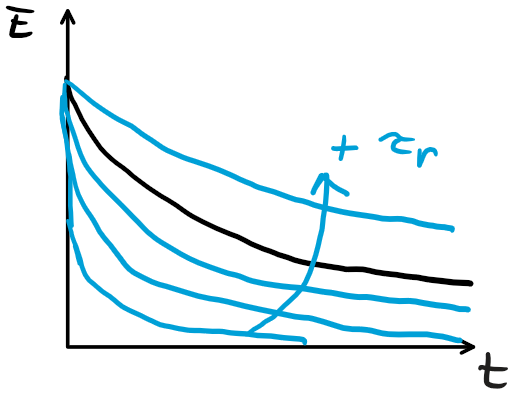
\includegraphics[width = 0.4\textwidth]{gfx/TempoRilassamento}}\quad	
\subfloat[][\emph{Comportamento al \eng{creep}}\label{fig:ComportamentoCreep}]%
{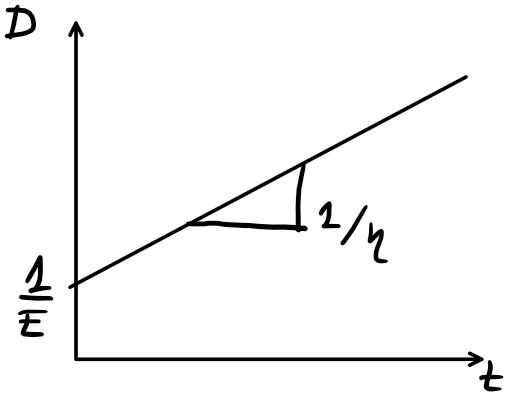
\includegraphics[width = 0.4\textwidth]{gfx/ComportamentoCreep}}	
\caption{Comportamenti del fluido di Maxwell}
\label{fig:ComportamentoMaxwell}
\end{figure}

\section{Modello di Kelvin-Voigt}

\begin{figure}
\centering
\subfloat[][\emph{Modello di \eng{Kelvin-Voigt}}\label{fig:KelvinVoigt}]%
{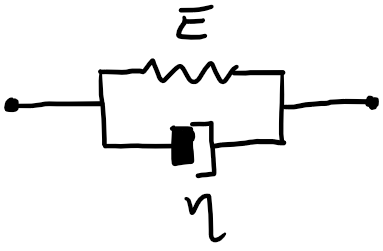
\includegraphics[width = 0.4\textwidth]{gfx/KelvinVoigt}}\quad
\subfloat[][\emph{Descrizione del modello}\label{def:KelvinVoigt}]%
{%
\begin{minipage}[b]{0.4\textwidth}
\begin{description}
\item[$E$] Modulo di Young della molla.
\item[$\eta$] Viscosità elemento dissipativo.
\end{description}
\end{minipage}%
}		
\caption{Modello di \eng{Kelvin-Voigt}}
\label{des:KelvinVoigt}
\end{figure}

La deformazione dell'elemento deve essere uguale per i due rami di molla e smorzatore.
Lo sforzo totale sarà pari alla somma degli sforzi dei due.
\begin{equation}
\begin{split}
\sigma = \sigma_1 + \sigma_2\\
\sigma_1 = E \epsilon_1, \quad \sigma_2 = \eta \dot{\epsilon}_2
\end{split}
\end{equation}
Ne deriva:
\begin{equation}
\sigma = E \epsilon + \eta \dot{\epsilon}
\end{equation}
\subsection{Prova di \eng{creep}}
\begin{equation}
\sigma = \bar{\sigma} \quad \forall t > 0
\end{equation}
Da cui:
\begin{equation}
\eta \dot{\epsilon} + E \epsilon = \bar{\sigma} \Rightarrow \dot{\epsilon} + \frac{E}{\eta}\epsilon = \frac{\bar{\sigma}}{\eta}
\end{equation}
Da cui la condizione iniziale per $\epsilon(0) = 0$
Il comportamento in questo caso se si applica un carico istantaneo si dovrebbe avere una deformazione della sola molla.
Siccome i due elementi sono in parallelo, prevale che: essendo lo smorzatore infinitamente rigido, allora la deformazione sarà nulla.

\begin{equation}
\begin{cases}
 \dot{\epsilon} + \frac{E}{\eta}\epsilon = \frac{\bar{\sigma}}{\eta} \rightarrow \epsilon(t) = \epsilon_h(t) + \epsilon_p(t)\\
\epsilon_p=\frac{\bar{\sigma}}{E}
\end{cases}
\end{equation}
Come si vede, l'equazione differenziale è non omogenea, dunque va calcolata:
\begin{equation}
\begin{split}
\dot{\epsilon}_h &+ \frac{E}{\eta}\epsilon_h = 0 \rightarrow \epsilon_h = K e^{-\frac{E}{\eta}t}\\
\epsilon(t) &= K e^{-\frac{E}{\eta}t}+\frac{\bar{\sigma}}{E} \rightarrow \epsilon(0) = K + \frac{\bar{\sigma}}{E} = 0 \rightarrow K = -\frac{\bar{\sigma}}{E}\\
\epsilon(t) &= -\frac{\bar{\sigma}}{E}e^{\frac{E}{\eta}t}+\frac{\bar{\sigma}}{E} = \frac{\bar{\sigma}}{E}\left(1-e^{-\frac{E}{\eta}t}\right)\\
D(t) &= \frac{\epsilon(t)}{\bar{\sigma}} = \frac{1}{E}\left(1-e^{-\frac{E}{\eta}t}\right) = D_{\infty}\left(1-e^{-\frac{t}{\tau_c}}\right)
\end{split}
\end{equation}
Dove, $\tau_c = \frac{\eta}{E}$ è il tempo di ritardo.

È un solido viscoelastico perché la cedevolezza è superiormente limitata.
Il materiale è istantaneamente rigido: risponde alla sollecitazione istantanea in maniera rigida.
Si osserva che però il modello è patologico perché:
per il comportamento a rilassamento: $\epsilon(t) = \bar{\epsilon}$ allora,
\begin{equation}
\sigma = E\epsilon + \eta \dot{\epsilon} = E \bar{\epsilon}
\end{equation}
Da cui:
\begin{equation}
E(t) = \frac{\sigma(t)}{\bar{\epsilon}} = E
\end{equation}
Non è accettabile che il modello di rilassamento resti costante.

\section{Modello \eng{Zener}, solido a tre parametri}

\begin{figure}
\centering
\subfloat[][\emph{Modello Zener}\label{fig:ModelloZener}]%
{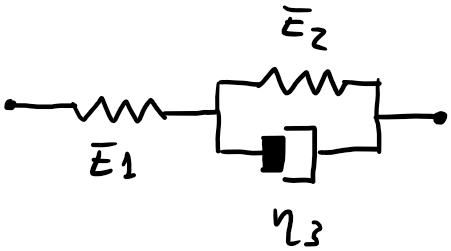
\includegraphics[width = 0.4\textwidth]{gfx/Zener}}\quad
\subfloat[][\emph{Parametri modello Zener}\label{prm:Zener}]%
{%
\begin{minipage}[b]{0.4\textwidth}
\begin{equation}
\begin{split}
\sigma_1 = E_1\epsilon_1 \quad &\epsilon_2 = \epsilon_3 = \epsilon_{23}\\
\sigma_2 = E \epsilon_2 \quad &\epsilon = \epsilon_1 + \epsilon_{23}\\
\sigma_3 = \eta_3 \dot{\epsilon}_3 \quad &
\end{split}
\end{equation}
\end{minipage}%
}
\caption{Modello e parametri del fluido Zener}
\label{def:Zener}		
\end{figure}

Da cui lo sforzo può esser descritto come:
\begin{equation}
\sigma = \sigma = \sigma_2 + \sigma_3
\end{equation}
Allora:
\begin{equation}
\begin{split}
\dot{\epsilon} &= \dot{\epsilon}_1 + \dot{\epsilon}_3 = \frac{\dot{\sigma}_1}{E_1} + \frac{\sigma_3}{\eta_3} = \frac{\dot{\sigma}}{E_1} + \frac{\sigma - \sigma_2}{\eta_3} = \frac{\dot{\sigma}}{E_1} + \frac{\sigma}{\eta_3} - \frac{E_2 \epsilon_2}{\eta_3}\\
&= \frac{\dot{\sigma}}{E_1} + \frac{\sigma}{\eta_3} - \frac{E_2}{\eta_3}(\epsilon - \epsilon_1) = \frac{\dot{\sigma}}{E_1} + \frac{\sigma}{\eta_3} - \frac{E_2}{\eta_3}\epsilon + \frac{E_2}{\eta_3}\frac{\sigma_1}{E_1}\\
&= \frac{\dot{\sigma}}{E_1} + \frac{\sigma}{\eta_3} - \frac{E_2\epsilon}{\eta_3} + \frac{E_2}{\eta_3}\frac{\sigma}{E_1}\\
\frac{\dot{\sigma}}{E} &+ \frac{1}{\eta_3}\left(1 + \frac{E_2}{E_1}\right)\sigma = \dot{\epsilon} + \frac{E_2}{\eta_3}\epsilon
\end{split}
\end{equation}

\subsection{Prova di \eng{creep}}
\begin{equation}
\dot{\epsilon} + \frac{E_2}{\eta_3}\epsilon = \frac{1}{\eta_3}\left(1+\frac{E_2}{E_1}\right)\bar{\sigma}
\end{equation}
Da cui la condizione iniziale $\epsilon(0) = \frac{\bar{\sigma}}{E_1}$
Resta un'equazione differenziale del primo ordine non omogenea, al solito la soluzione sarà combinazione della soluzione dell'omogenea e una soluzione particolare.
\begin{equation}
\begin{split}
\epsilon_p(t) &= cost = \frac{E_2}{\eta_3}\epsilon_p = \frac{1}{\eta_3}\left(1+\frac{E_2}{E_1}\right)\bar{\sigma}\\
\epsilon_p &= \left(\frac{1}{E_2} + \frac{1}{E_1}\right)\bar{\sigma}\\
\epsilon_h(t) &= K e^{-\frac{E_2}{\eta_3}t}\\
\epsilon(t) &= K e^{-\frac{E_2}{\eta_3}t} + \left(\frac{1}{E_2} + \frac{1}{E_1}\right)\bar{\sigma}\\
\epsilon(0) &= K + \left(\frac{1}{E_2} + \frac{1}{E_1}\right)\bar{\sigma} = \frac{\bar{\sigma}}{E_1} \Rightarrow K = -\frac{\bar{\sigma}}{E_2}\\
\epsilon(t) &= -\frac{\bar{\epsilon}}{E_2}e^{-\frac{E_2}{\eta_3}t} + \left(\frac{1}{E_2} + \frac{1}{E_1}\right)\bar{\sigma}\\
\epsilon(t) &= \frac{1}{E_1}\bar{\epsilon} + \frac{\bar{\sigma}}{E_2}\left(1-e^{-\frac{E_2}{\eta_3}t}\right)
\end{split}
\end{equation}
E:
\begin{equation}
D(t) = \frac{\epsilon(t)}{\bar{\sigma}} = \frac{1}{E_1} + \frac{1}{E_2}\left(1-e^{-\frac{E_2}{\eta_3}t}\right)
\end{equation}
Resta valido che:
\begin{equation}
\begin{split}
t \rightarrow 0 \quad &D(0) = \frac{1}{E_1}\\
t \rightarrow \infty \quad &D(\infty) = \frac{1}{E_1} + \frac{1}{E_2}\\
D(t) &= D_0 + (D_{\infty} - D_0) \left(1 - e^{-\frac{t}{\tau_c}}\right)
\end{split}
\end{equation}
Con $\tau_c = \frac{\eta_3}{E_2}$ tempo di ritardo della cedevolezza.

\begin{figure}
\centering
\subfloat[][\emph{Funzione di cedevolezza in funzione del tempo per il modello di \eng{Zener}}\label{fig:CedevolezzaZener}]%
{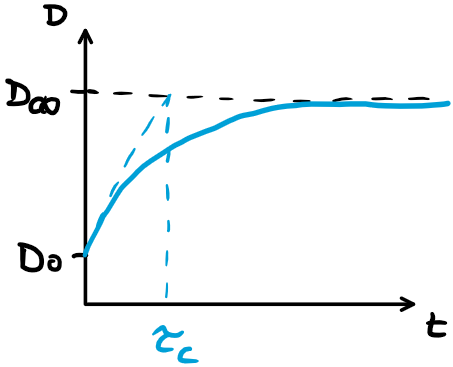
\includegraphics[width = 0.4\textwidth]{gfx/CedevolezzaZener}}	\quad
\subfloat[][\emph{Modulo di rilassamento per il modello \eng{Zener}}\label{fig:RilassamentoZener}]%
{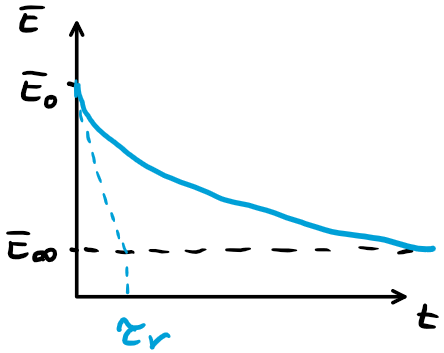
\includegraphics[width = 0.4\textwidth]{gfx/RilassamentoZener}}	
\caption{Modello \eng{Zener}}
\label{fig:ModelloZener}
\end{figure}

Il materiale è un solido viscoelastico perché la cedevolezza di \eng{creep} è superiormente limitata.

Si nota negli altri comportamenti come se fosse elastico. La parte dissipativa appare lontano dai limite. in un certo senso, dipende dal ritardo elastico: se $\eta_3\downarrow$ allora il materiale sarà più a comportamento elastico: se $\eta_3\uparrow$ il materiale risulterà più dissipativo.

\subsection{Prova di rilassamento}
Allora imponiamo $\epsilon = \bar{\epsilon}$.
\begin{equation}
\begin{cases}
\frac{\dot{\sigma}}{E_1} + \frac{1}{\eta_3}\left(1 + \frac{E_2}{E_1}\right)\sigma = \frac{E_2}{\eta_3}\bar{\epsilon}\\
\textup{Condizione iniziale: } \sigma(0) = E_1\bar{\epsilon}\\
\end{cases}
\end{equation}
La soluzione dell'equazione differenziale:
\begin{equation}
\begin{split}
\sigma(t) &= \sigma_h(t) + \sigma_p(t)\\
\sigma_p(t) &= \sigma_p \rightarrow \sigma_p = \frac{E_1 E_2}{E_1+E_2}\bar{\epsilon}\\
\sigma_h(t) &= \frac{\dot{\sigma}}{E_1} + \frac{1}{\eta_3}\left(1+\frac{E_2}{E_1}\right)\sigma = 0\\
&= \dot{\sigma} + \frac{1}{\eta_3}\left(E_1 + E_2\right)\sigma = 0\\
&= K e^{-\frac{E_1+E_2}{\eta_3}t}\\
\sigma(t) &= Ke^{-\frac{E_1+E_2}{\eta_3}t} + \frac{E_1E_2}{E_1+E_2}\bar{\epsilon}\\
\sigma(0) &= K + \frac{E_1E-2}{E_1 + E_2}\bar{\epsilon} = E_1\bar{\epsilon}\\
&\Rightarrow K = E_1\bar{\epsilon}-\frac{E_1E_2}{E_1+E_2}\bar{\epsilon} = \frac{E_1^2}{E_1+E_2}\bar{\epsilon}\\
\sigma(t) &= \frac{E_1^2}{E_1+E_2}\bar{\epsilon}e^{-\frac{E_1+E_2}{\eta_3}t}+\frac{E_1E_2}{E_1+E_2}\bar{\epsilon}
\end{split}
\end{equation}
Da cui:
\begin{equation}
E(t) = \frac{\sigma(t)}{\bar{\epsilon}} = \frac{E_1^2}{E_1+E_2}e^{-\frac{E_1+E_2}{\eta_3}t}+\frac{E_1E_2}{E_1+E_2}\bar{\epsilon}
\end{equation}
Ai limiti:
\begin{equation}
\begin{split}
t \rightarrow 0 \quad &E_0 = \frac{E_1E_2}{E_1+E_2}+\frac{E_1^2}{E_1+E_2} = E_1\\
t \rightarrow \infty \quad &E_{\infty} = \frac{E_1E_2}{E_1+E_2}\\
E(t) &= E_{\infty} + (E_0 - E_{\infty})e^{-\frac{t}{\tau_r}}
\end{split}
\end{equation}
Con $\tau_r = \frac{\eta_3}{E_1+E_2}$ tempo di rilassamento.

Si cedevolezza che modulo sono funzioni esponenziali, in entrambi i casi limitati e non arrivano ne a zero che infinito.

Il modello \eng{Zener} può avere un'altra conformazione con lo stesso risultato: non è esattamente lo stesso, la forma della risposta sarà la stessa, ma i parametri saranno utilizzati diversamente.